\chapter{FOPT6 - Webbasierte Client-Server-Anwendungen in Java (Programmierung verteilter Anwendungen 2)}

\section{Lehrstoff}
Das Skript FOPT6 bezieht sich auf folgende Inhalte im Buch:

\begin{tcolorbox}[colback=white!20,color=white]
    \begin{enumerate}
        \setcounter{enumi}{13}
        \item \textbf{Das HTTP-Protokoll}
        \begin{itemize}
            \item[] Kapitel 8
            \item[] Abschnitt 8.1
        \end{itemize}

        \item \textbf{Einführende Servlet-Beispiele}
        \begin{itemize}
            \item[] Abschnitt 8.2
        \end{itemize}

        \item \textbf{Parallelität bei Servlets}
        \begin{itemize}
            \item[] Abschnitt 8.3
        \end{itemize}

        \item \textbf{Sessions und Cookies}
        \begin{itemize}
            \item[] Abschnitt 8.4
        \end{itemize}

        \item \textbf{JSF (Java Server Faces)}
        \begin{itemize}
            \item[] Abschnitt 8.8
        \end{itemize}

        \item \textbf{Schlussbemerkung}
        \begin{itemize}
            \item[] Abschnitt 8.11
        \end{itemize}

    \end{enumerate}
\end{tcolorbox}

\newpage

\section{Das HTTP-Protokoll}

Bei webbasierten Anwendungen wird die Client-Seite durch einen Web-Browser realisiert, auf der Server-Seite wird ein Web-Server wie bspw. \textit{Apache Tomcat}\footnote{
    \url{https://tomcat.apache.org} - abgerufen 3.2.2024
} benutzt.\\

\noindent
Der Web-Server liefert statische Dateien aus oder Seiten, die Programmcode enthalten, der auf dem Client ausgeführt wird (bspw. \textit{JavaScript}).\\

\noindent
Der Client kann auch über den Server ausgeführte Programme anfordern, die entsprechende Daten für den Client generieren, wie bspw. \textbf{Servlets}.\\

\noindent
Um mit einem Server zu kommunizieren, baut der Client über \textbf{TCP} eine Verbindung mit dem Server auf:\\
Über das \textbf{HTTP-Protokoll}\footnote{
Bestandteilt der Anwendungsschicht - s. \url{https://en.wikipedia.org/wiki/HTTP} - abgerufen 3.2.2024
} werden dann Anfragen und Antworten zwischen Client und Server verhandelt; Antworten können über auf dem Server laufende Programme dynamisch generierte Seiteninhalte sein.\\

\noindent
\textbf{HTTP} (\textit{HyperTextTransferProtocol})\footnote{
    s. a. ``RFC 9110 HTTP Semantics``: \url{https://www.rfc-editor.org/rfc/rfc9110.html} - abgerufen 4.2.2024
} ist ein ASCII-Protokoll auf Schicht 5 und für die Vermittlung webbasierter Dienste gedacht.

\begin{figure}
    \centering
    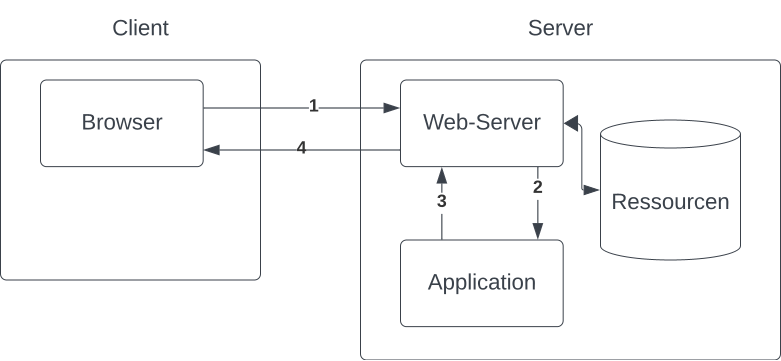
\includegraphics[scale=0.5]{chapters/fopt6/img/clientserver}
    \caption{Der Client erstellt über den Webbrowser eine TCP-Verbindung zu dem Webserver, wobei die Adressinformationen in der URL festgelegt sind.
    Der Webserver kann nun in seiner Antwort sowohl statische Ressourcen als auch dynamisch generierte Daten bereitstellen.
    Syntax und Semantik der Anfrage und Antwort ist über das HTTP-Protokoll definiert (Quelle: in Anlehnung an \cite[402, Bild 8.1]{Oec22})}
    \label{fig:clientserver}
\end{figure}

\subsection{GET}

Über eine \textbf{URL} (\textit{Universal Resource Locator}\footnote{
s. \url{https://en.wikipedia.org/wiki/URL} - abgerufen 3.2.2024
}) wird über den Browser eine Ressource angefordert.

\begin{tcolorbox}[enlarge top by=0.5cm,enlarge bottom by=0.5cm]
    Eine \textbf{URL} ist eine \textbf{URI} (\textit{Uniform Resource Identifier}\footnote{
        s. \url{https://en.wikipedia.org/wiki/Uniform_Resource_Identifier} - abgerufen 3.2.2024
    }) und enthält u.a. weitere Informationen zur Lokalisierung der Ressource - bspw. durch die Angabe des Protokolls, über das die Ressource beschafft werden soll\footnote{s. ``RFC 3986 - 1.1.3.  URI, URL, and URN``: \url{https://datatracker.ietf.org/doc/html/rfc3986#section-1.1.3} - abgerufen 3.2.2024}.
\end{tcolorbox}

\noindent
Der an den Server übermittelte \textbf{GET}-Request besteht aus der Angabe der angeforderten Ressource und dem Protokoll, das verwendet wird:

\begin{minted}[]{http}
GET /resource.html HTTP/1.1
\end{minted}
\\

$\rightarrow$ Ein \textbf{GET}-Request besteht aus beliebig vielen Zeilen.
Mit einer Leerzeile wird das Ende des Request angezeigt.\\

\noindent
Eine \textbf{HTTP-Response} enthält wieder Kopfdaten (\textbf{Header}) und den \textbf{Body}, der leer sein kann.\\
Header und Body sind durch eine Leerzeile voneinander getrennt\footnote{
    s. \url{https://www.rfc-editor.org/rfc/rfc7230#section-3} - abgerufen 3.2.2024
}.\\
Weitere Leerzeilen im Body haben keine weitere Bedeutung für das Protokoll und gehören zum Inhalt der angeforderten Ressource.\\

\noindent
Der Client kann weitere Daten anfordern, bspw. wenn in der ausgelieferten HTML-Seite Bilder oder andere statische Ressourcen vorkommen.\\
Bei \textbf{HTTP/1.0} muss der Client für jede Ressource eine neue \textbf{TCP}-Verbindung aufbauen.\\
Nutzt der Client hingegen \textbf{HTTP/1.1}, hält der Server genau diese Verbindung offen.
Über diese Verbindung kann der Client weitere Daten anfordern.

\begin{itemize}
    \item Bei der Verwendung von \textbf{HTTP/1.1} muss außerdem in der zweiten Zeile der Anfrage der Zielhost stehen, damit ein Server, der {ggf.} mehrere Domains hostet, die Anfrage an die richtige Domain weiterleitet\footnote{s. ``RFC 7320 - 5.4.  Host``: \url{https://www.rfc-editor.org/rfc/rfc7230#section-5.4} - abgerufen 3.2.2024}.
    \begin{minted}[]{http}
GET /index.php HTTP/1.1
Host: www.conjoon.org
    \end{minted}
    \item Wird der Header \textit{Connection: keep-alive}\footnote{
    s. ``RFC 2068 - 19.7.1 Compatibility with HTTP/1.0 Persistent Connections``: \url{https://www.rfc-editor.org/rfc/rfc2068#section-19.7.1} - abgerufen 3.2.2024
    } mitgesendet, teilt der Client dem Server mit, dass die Verbindung zum Herunterladen weiterer Daten geöffnet bleiben soll (\textit{close} als default für HTTP/1.0-Requests, \textit{keep-alive} als default für HTTP/1.1-Requests).
    \item Bei einer HTTP-Response weist die Antwort-Zeile \textit{Connection: close} daraufhin, dass die Verbindung nicht persistent ist und mit der Bearbeitung der Antwort geschlossen wird\footnote{
    s. ``RFC 2068 - 14.10 Connection``: \url{https://www.rfc-editor.org/rfc/rfc2068#section-14.10} - abgerufen 3.2.2024
    }.
\end{itemize}

\subsection{Formulare in HTML}

\textit{<form>...</form>} wird für Formulare in HTML genutzt, in \textit{action} steht die URL, an der die Formulardaten gesendet werden sollen, mit \textit{method} kann man die HTTP-Methode angeben, die zum Senden des Formulars genutzt werden soll\footnote{
s. ``<form>: The Form element``:\url{https://developer.mozilla.org/en-US/docs/Web/HTML/Element/form} - abgerufen 3.2.2024
}.\\

\noindent
\textbf{radio}-inputs erhalten alle dasselbe \textit{name}-Attribut, um sie zu einer Gruppe zusammenzuführen.\\

\noindent
Fehlt für eine \textbf{checkbox} die Selektion, wird sie bei der Übertragung der Formulardaten nicht berücksichtigt.
Ist das \textit{value}-Attribut für die Checkbox gesetzt und wurde die Checkbox selektiert, enthalten die Request-Daten den Inhalt von \textit{value}, ansonsten standardmäßig den Wert \textit{on}:

\blockquote[{\url{https://developer.mozilla.org/en-US/docs/Web/HTML/Element/input/checkbox} - abgerufen 3.2.2024, Hervorherbungen ausgelassen}]{
    If the value attribute was omitted, the default value for the checkbox is on, so the submitted data in that case would be subscribe=on.
}

\subsection{POST}

Nutzt man \textbf{GET} zur Übermittlung von Formulardaten, werden die Daten als Query-String an die URL gehangen.\\

\noindent
\textbf{POST} schickt die Formulardaten im Body an die in \textit{action} angegebene URL.

\begin{itemize}
    \item Vorteile \textbf{GET}: Formulardaten können mit der URL gespeichert werden, bei \textbf{POST} geht das nicht, da diese im Body verborgen sind
    \item Nachteile \textbf{GET}: bei \textbf{GET} ist die Länge der eingegebenen Formulardaten begrenzt, bei \textbf{POST} nicht.
    \begin{tcolorbox}[colback=red!20,color=white,title=Anmerkung]
    Die Aussage bzgl. der Begrenzung von \textbf{GET/POST} findet sich in \cite[409]{Oec22}.\\
    Tatsächlich ist die Länge nicht begrenzt per Spezifikation\footnote{``RFC 7230 - 3.1.1.  Request Line``: \url{https://datatracker.ietf.org/doc/html/rfc7230#section-3.1.1} - abgerufen 3.2.2024}. \\
    Es wird aber empfohlen, Request URIs abzuweisen, die zu lang sind\footnote{siehe bspw. ``RFC 2616 - 10.4.15 414 Request-URI Too Long``: \url{https://datatracker.ietf.org/doc/html/rfc2616#section-10.4.15} - abgerufen 3.2.2024
    }.\\
    Auch für \textbf{POST} wird in den Spezifikationen keine max. Länge vorgegeben.
    Allerdings kann die max. akzeptierte Länge des Bodys eines POST-Requests durch den Web-Server begrenzt werden\footnote{
        ``RFC7231 - 6.5.11.  413 Payload Too Large``: \url{https://www.rfc-editor.org/rfc/rfc7231#section-6.5.11} - abgerufen 3.2.2024
    }.\\
    Beides ist sinnvoll, um einer Überlastung des Webservers durch zu große Anfrage-Längen vorzubeugen.
    \end{tcolorbox}
\end{itemize}

\subsection{Format von HTTP-Anfragen und -Antworten}

Eine HTTP-Anfrage hat grundsätzlich folgende Struktur\footnote{
Es ist grundsätzlich möglich, bei GET-Requests den Body mitzuschicken.
    Allerdings rät RFC 9110 davon ab: ``A client \textbf{SHOULD NOT} generate content in a GET request unless it is made directly to an origin server that has previously indicated, in or out of band, that such a request has a purpose and will be adequately supported. An origin server \textbf{SHOULD NOT} rely on private agreements to receive content, since participants in HTTP communication are often unaware of intermediaries along the request chain.`` (Hervorhebungen i.O., \url{https://www.rfc-editor.org/rfc/rfc9110#section-9.3.1-6} - abgerufen 3.2.2024)
}:

\begin{minted}[]{text}
<methode> <uri> HTTP/<version>
<headername>: <headerwert>
...
<headername>: <headerwert>
<newline>
<body>
\end{minted}

Die Antwort sieht i.A. folgendermaßen aus:

\begin{minted}[]{text}
HTTP/<version> <StatusCode> <StatusText>
<headername>: <headerwert>
...
<headername>: <headerwert>
<newline>
<body>
\end{minted}

\subsection*{``Content-Length`` Header}
Bei \textbf{POST} nutzt der Server die Verbindung, die der Client zur Anfrage aufgebaut hat, um die Antwort zu senden.\\
Der Server muss wissen, wann er den kompletten Datenteil gelesen hat, bevor er mit der Antwort beginnt.\\
Bis zum Verbindungsende kann nicht gelesen werden, sonst kann keine Antwort gesendet werden.\\
Trennzeichen sind für den Body nicht ausgemacht.\\
Nach $n$-Zeichen, die der Client im Header über \textbf{Content-Length} spezifiziert, geht der Server davon aus, dass die Anfrage nach der Leerzeile (Trennzeichen Header / Body) genauso viele Daten enthält.\\
Sind diese $n$ Daten gelesen, beginnt der Server mit der Aufbereitung der Antwort an den Client\footnote{
s.a. Skript FOPT6 Übung 14.2
}.



\section{Einführende Servlet-Beispiele}

\subsection{Allgemeine Vorgehensweise}

Zur Erstellung eines Servlets muss die Klasse von \begin{center}\code{jakarta.servlet.http.HttpServlet}\footnote{
    Das Buch verwendet bereits die Klassen aus dem \textit{Jakarta EE}, die Skripte benutzen noch die \textit{javax.*}-Namensräume
}\footnote{
    ``Class HttpServlet``: \url{https://jakarta.ee/specifications/servlet/6.0/apidocs/jakarta.servlet/jakarta/servlet/http/httpservlet} - abgerufen 3.2.2024
}\end{center} abgeleitet werden.\\

\noindent
Die Methoden \begin{center}\code{#doGet(request:HttpServletRequest, response:HttpServletResponse):void}\end{center} sowie \begin{center}\code{#doPost(request:HttpServletRequest, response:HttpServletResponse):void}\end{center} sind in der Basisklasse vorimplementiert und liefern per Default einen $405$ Status Code\footnote{
    ``405 Method Not Allowed``: \url{https://developer.mozilla.org/en-US/docs/Web/HTTP/Status/405} - abgerufen 3.2.2024
}, sofern die Methoden in einer abgeleiteten Klasse nicht sinnvoll überschrieben sind\footnote{
die Methode \textit{service} in der \textit{HttpServlet}-Klasse funktioniert als Dispatcher und leitet - basierend auf der ermittelten Request-Methode (\textbf{GET}, \textbf{POST}, \textbf{PUT}...) an die entsprechende \textit{doX}-Methode weiter.
}:

\noindent
Die Methoden \code{init()} (Servlet wird vom Servlet-Container aktiviert) / \code{destroy()} (Servlet wird vom Servlet-Container deaktiviert) können ebenfalls noch überschrieben werden.\\

\noindent
\code{init()} wird beim Hochfahren des Webservers, der Installation der Web-Anwendung oder beim Aufruf des Servlets aufgerufen.
\code{destroy()} wird aufgerufen, bevor das Servlet ``vernichtet`` wird, also beim Herunterfahren des Webservers oder beim Undeployment\footnote{
generell kann in dem Context zwischen \textit{Deployment, Redeployment, Undeployment} unterschieden werden.
} der Web-Anwendung. \\

\noindent
Der Pfad, unter dem ein Servlet letztendlich auf dem Webserver erreichbar ist, kann mit Hilfe der Annotation \code{@WebServlet} angegeben werden, bspw. \begin{center}\code{@WebServlet(``/hello-world``)}\end{center} wobei der String mit einem ``/`` beginnen muss\footnote{
    ``Annotation Type WebServlet``: \url{https://jakarta.ee/specifications/servlet/6.0/apidocs/jakarta.servlet/jakarta/servlet/annotation/webservlet} - abgerufen 3.2.2024
}.\\

\noindent
Ein Servlet benötigt keine \code{main}-Methode, die \code{do...()}-Methoden werden automatisch aufgerufen (durch den sogenannten \textbf{Servlet-Container} des Webservers).

\begin{tcolorbox}[enlarge top by=0.5cm,enlarge bottom by=0.5cm]
    Es ist ohne Weiteres möglich, die \code{do...()}-Methoden untereinander aufzurufen, bspw. kann \code{doPost()} die Methode \code{doGet()} aufrufen - vorausgesetzt, die Parameter (\code{HttpServletRequest} und \code{HttpServletResponse}) werden korrekt übergeben.
\end{tcolorbox}\\

\noindent
Der Parameter \code{HttpServletResponse} stellt einen \code{java.io.PrintWriter}\footnote{
mittels \textit{getWriter()}. S. ``getWriter``: \url{https://jakarta.ee/specifications/servlet/6.0/apidocs/jakarta.servlet/jakarta/servlet/servletresponse#getWriter()} - abgerufen 3.2.2024
} zur Verfügung, mit dem man den \code{OutputStream} (ASCII) der Response verändern kann.

\begin{tcolorbox}[enlarge top by=0.5cm,enlarge bottom by=0.5cm]
    Man sollte stets daran denken, über das \code{HttpServletResponse}-Argument auch den \textbf{Content-Type} der Response zu setzen:
    \begin{minted}[mathescape,
        numbersep=5pt,
        gobble=2,
        frame=none,
        framesep=2mm]{java}
    response.setContentType("text/html");
    \end{minted}\\
\end{tcolorbox}

\noindent
In dem Verzeichnis \textit{webapp} liegen statische Ressourcen, die von der Webapplikation ausgeliefert werden können.\\
Das Verzeichnis \textit{WEB-INF}, das dortdrin liegt, ist von außen nicht erreichbar.\\


\noindent
Der Parameter \code{HttpServletRequest} besitzt eine Methode \begin{center}\code{getParameter(name:String): String}\end{center} über den man an \textbf{GET}- / \textbf{POST-Parameter} kommt.\\

\noindent
Mit \code{getParameterNames()} kommt man an alle Parameternamen des Requests - da unter einem Parameternamen mehrere Werte vorhanden sein können  (bspw. \code{Post name=1} und \code{/foo?name=2}) kann man mit \begin{center}\code{getParameterValues(name: String): String[]}\end{center} auf ein Feld dieser Werte zugreifen.\\

\noindent
Darüberhinaus bietet \code{HttpServletRequest} noch die Methoden \code{getHeader()}, \code{getMethod()}, \code{getRemoteHost()}...\\

\noindent
Die Methoden \code{setStatus()} und \code{setHeader()} stehen im \code{HttpServletResponse} zur Verfügung.

\noindent
Ein Servlet wird beim (Re)deployment des Servers instanziiert, dieses Objekt wird  dann benutzt, um alle Anfragen zu bearbeiten, bis der Server neu deployed wird -  dass Objekt wird dann neu initialisiert.

\begin{tcolorbox}[enlarge top by=0.5cm,enlarge bottom by=0.5cm]
    \code{loadOnStartup=1} in \code{@WebServlet} sorgt dafür, dass das Servlet beim (Re)deploy initialisiert wird ($[0, .., n]$ sind als Werte erlaubt, mit denen die Startreihenfolge angegeben wird)\footnote{
        s. ``loadOnStartup``: \url{https://jakarta.ee/specifications/servlet/6.0/apidocs/jakarta.servlet/jakarta/servlet/annotation/webservlet#loadOnStartup()} - abgerufen 3.2.2024
    }.\\
    $-1$ ist default, und führt keine Initialisierung während des Starts durch.
    Das Servlet wird dann i.d.R. beim Aufruf initialisiert.
\end{tcolorbox}


\section{Parallelität bei Servlets}

Bei der Bearbeitung von Anfragen eines Servlets ist implizit Parallelität im Spiel - jede HTTP-Anfrage wird in einem eigenen Thread ausgeführt.

\begin{tcolorbox}[enlarge top by=0.5cm,enlarge bottom by=0.5cm]
Alle Anfragen arbeiten mit demselben Servlet-Objekt $\rightarrow$ pro Servlet-Klasse wird ein Objekt davon für den jeweiligen Context erzeugt.
\end{tcolorbox}


\subsection{Anwendungsglobale Daten}

Von unterschiedlichen Servlets kann auf ein und dasselbe Objekt zugegriffen werden, wenn es vorher über den \code{ServletContext} registriert wurde.\\
\code{getServletContext()} steht in \code{HttpServlet} zur Verfügung und liefert den \code{ServletContext}, in dem das Servlet läuft.\\
Über \code{getAttribute():Object} bzw.\\ \code{setAttribute(name:String, object:Object):void} können Objekte unter einem bestimmten Namen im \code{ServletContext} registriert werden.\\

\noindent
Die über \code{loadOnStartup} definierte Reihenfolge kann entscheidend sein beim Zugriff auf ein im \code{ServletContext} enthaltenes Attribut.\\
Wird ein Servlet mit \code{loadOnStartup=1} konfiguriert, und wird dort auf ein Attribut des \code{ServletContext} zugegriffen (bspw. in der \code{init()}), dessen Servlet\footnote{
lies: Das Servlet, dass das Attribut im \textit{ServletContext} registriert
} noch nicht initialisiert wurde, kann es zu Fehlern kommen.\\

\noindent
Neben der Registrierung eines Attributes über die \code{init()}-Methode im Servlet ist es auch möglich, über einen \code{ServletContextListener}\footnote{
    ``Interface ServletContextListener``: \url{https://jakarta.ee/specifications/servlet/6.0/apidocs/jakarta.servlet/jakarta/servlet/servletcontextlistener} - abgerufen 3.2.2024
} und der Annotation \code{@WebListener}\footnote{
``Annotation Type WebListener``: \url{https://jakarta.ee/specifications/servlet/6.0/apidocs/jakarta.servlet/jakarta/servlet/annotation/weblistener} - abgerufen 3.2.2024
} ein ``globales Objekt`` zu registrieren (sobald der \code{ServletContext} zur Verfügung steht; die Informationen hierüber enthält man in der Methode \code{contextInitialized()} des \code{ServletContextListener}).\\

\noindent
Über einen \code{ServletContextAttributeListener}\footnote{
    ``Interface ServletContextAttributeListener``: \url{https://jakarta.ee/specifications/servlet/6.0/apidocs/jakarta.servlet/jakarta/servlet/servletcontextattributelistener} - abgerufen 3.2.2024
} kann man sich (wieder mittels Annotation \code{@WebListener}) darüber informieren lassen, wann ein Attribut im \code{ServletContext} (de-)registriert wurde.

\section{Sessions und Cookies}

Da HTTP zustandslos ist, kann man einen Zustand mit Hilfe einer \textbf{Session} speichern, die den jeweiligen Benutzern einer Web-Anwendung eindeutig zugeordnet werden können\footnote{
Identifizierung mittels der IP ist nicht möglich, da mehrere Rechner in einem Netz hinter der gleichen IP angeschlossen sein können, bspw. bei der Verwendung eines Proxies (Adressumsetzung auf Schicht 5) oder bei der Verwendung von \textbf{NAT} (Network Address Translation, \textit{Adressenabbildung}), bei der ein Router über seine öffentliche IP Antworten auf Requests angeschlossener Clients empfängt, und an diese weiterleitet (Schicht 3) (vgl.~\cite[425]{Oec22}).
}.\\

\noindent
\code{HttpServletRequest} bietet hierzu die Methode \code{getSession()}, die, sofern keine Session (Typ: \code{HttpSession}\footnote{
``Interface HttpSession``: \url{https://jakarta.ee/specifications/servlet/6.0/apidocs/jakarta.servlet/jakarta/servlet/http/httpsession} - abgerufen 3.2.2024
}) existiert, eine neue erzeugt (falls Parameter \code{create:boolean} den Wert \code{true} besitzt oder die Methode ohne Parameter aufgerufen wurde; \code{false} erzeugt keine neue Session und liefert \code{null} zurück, falls keine existiert).\\

\noindent
Über \code{setAttribute()} / \code{getAttribute()} \code{removeAttribute()} (definiert in\\ \code{HttpSession}) lassen sich Sitzungsdaten ändern.\\

\noindent
Die Methode \code{invalidate()} von \code{HttpSession} löscht explizit eine Session, alternativ kann man mittels \code{setMaxInactiveInterval} angeben, wie lange die Sitzung maximal inaktiv sein darf, bevor sie gelöscht wird, damit der Speicher des Servers nicht unnötig belastet wird.

\begin{tcolorbox}[enlarge top by=0.5cm,enlarge bottom by=0.5cm]
Auch Sitzungsdaten müssen synchronisiert werden, da ein Anwender parallel mehrere Tabs offen haben kann.\\
Hierzu muss man nicht zwingend die entsprechende \textit{do*}-Methode synchronisieren - unter Umständen reicht es, über das \code{synchronized}-Statement das Session-Objekt zu sperren, und dann in dem nachfolgenden Block mit der Session zu arbeiten:

\begin{minted}[mathescape,
    numbersep=5pt,
    gobble=2,
    frame=none,
    fontsize=\small,
    framesep=2mm]{java}
    protected void doGet(HttpServletRequest request, HttpServletResponse response) {

        HttpSession session = request.getSession(false); // keine neue Session erzeugen
        if (session != null) {
            synchronized (session) { // synchronized-statement, damit nicht das Servlet
                                     // bei gleichzeitigen doGet-Aufrufen gesperrt
                                     // werden muss
                String value = (String)session.getAttribute("value");
                session.setAttribute("value", value + " set, done.");
            }
        }

    }

\end{minted}\\

\end{tcolorbox}\\

\noindent
Es existieren wie für \textbf{ServletContext} auch Listener für \textbf{Sessions}:\\
Der \code{HttpSessionListener}\footnote{
    ``Interface HttpSessionListener``: \url{https://jakarta.ee/specifications/servlet/6.0/apidocs/jakarta.servlet/jakarta/servlet/http/httpsessionlistener} - abgerufen 3.2.2024
} erlaubt mittels \code{sessionCreated()} / \code{sessionDestroyed()}\footnote{``Receives notification that a session is about to be invalidated.`` (\url{https://jakarta.ee/specifications/servlet/6.0/apidocs/jakarta.servlet/jakarta/servlet/http/httpsessionlistener#sessionDestroyed(jakarta.servlet.http.HttpSessionEvent)} - abgerufen 3.2.2024)} das Überwachen einzelner Sessions (die Methoden erhalten ein Argument vom Typ \code{HttpSessionEvent}, dessen Methode \code{getSession()} erlaubt den Zugriff auf die \textbf{Session}); der Listener kann wieder mit \code{@WebListener} annotiert werden.

\begin{tcolorbox}[enlarge top by=0.5cm,enlarge bottom by=0.5cm]
Es können mehrere Listener gleichen Typs parallel existieren.
\end{tcolorbox}\\

\noindent
Wie beim  \code{ServletContextAttributeListener} gibt es auch den\\ \code{HttpSessionAttributeListener}\footnote{``Interface HttpSessionAttributeListener``: \url{https://jakarta.ee/specifications/servlet/6.0/apidocs/jakarta.servlet/jakarta/servlet/http/httpsessionattributelistener} - abgerufen 3.2.2024
} zum Überwachen von Attributänderungen der Sitzungsdaten: \code{attributeAdded()}, \code{attributeReplaces()}, \code{attributeRemoved()}\\

\noindent
Sessions werden in der Regel über \textbf{Cookies} realisiert, deren Kennung\\ \textbf{JSESSIONID} auf dem Client gespeichert ist und bei Anfragen im \textbf{Cookie-Header} mitgesendet werden.\\
$\rightarrow$ Die Anforderung zur Speicherung der Cookie-Daten kommt \textit{über den Response} im Header \code{Set-Cookie}\footnote{
    `´Set-Cookie``: \url{https://developer.mozilla.org/en-US/docs/Web/HTTP/Headers/Set-Cookie}
} (die Kennung lässt sich auch über die Methode \code{getId()} von \code{HttpSession} erfragen).\\

\noindent
Sitzungsdaten werden i.d.R. im Speicher des Webservers in einer Art \code{HashMap} gespeichert; jede Sitzungs-Id hat ein Sitzungs-Objekt zugeordnet, in der die Attribut-Werte-Paare gespeichert sind.\\

$\rightarrow$ Beim Aufruf \code{getSession()} wird geprüft, ob der \code{Cookie}-Header\footnote{
    ``Cookie``: \url{https://developer.mozilla.org/en-US/docs/Web/HTTP/Headers/Cookie} - abgerufen 3.2.2024
} vorhanden ist.
Die Sitzungs-Id wird dann verwendet, um in der Tabelle nach einem assoziierten Sitzungsobjekt zu schauen - soll eine neue Sitzung erzeugt werden, wird dies entsprechend automatisch in der Response im \code{Set-Cookie}-Header vermerkt.\\

\noindent
Bei horizontaler Skalierung können Sitzungsobjekte i.d.R nicht geteilt werden unter den beteiligten Webservern - hier eignet sich eine zentrale Speicherung der Sitzungsdaten, bspw. in einer Datenbank (vgl.~\cite[433]{Oec22}).

\subsection{Direkter Zugriff auf Cookies}\label{sec:cookieaccess}
Die Servlet-Klassenbibliothek erlaubt auch einen direkten Zugriff auf Cookies.\\

\noindent
$\rightarrow$ die Klasse \code{Cookie}\footnote{
``Class Cookie``: \url{https://jakarta.ee/specifications/servlet/6.0/apidocs/jakarta.servlet/jakarta/servlet/http/cookie} - abgerufen 3.2.2024
} mit dem Konstruktor \code{Cookie(name: String, value: String)} erlaubt das direkte Erzeugen von Cookie-Objekten, die dann mittels \code{addCookie(cookie: Cookie): void} (der Klasse \code{HttpServletResponse}) bzw. \code{getCookies(): Cookie[]} (der Klasse \code{HttpServletRequest}) ausgelesen werden können.\\

\noindent
Cookies, die die Lebensdauer einer Browsersitzung überdauern sollen, sollten mittels \code{setMaxAge(expiry:int):void}\footnote{
    ``Sets the maximum age in seconds for this Cookie.`` (\url{https://jakarta.ee/specifications/servlet/6.0/apidocs/jakarta.servlet/jakarta/servlet/http/cookie#setMaxAge(int)} - abgerufen 3.2.2024)
} konfiguriert werden (die Browsereinstellungen des Nutzers haben hier aber Vorrang).


\begin{tcolorbox}
    Session-Cookies werden i.d.R. nach den Schliessen des Browsers gelöscht.\\ Um dieses Verhalten für ``reguläre`` Cookies umzusetzen, kann man über die Methode \code{setMaxAge()} einen negativen Wert übergeben\footnote{der Wert $0$ veranlaßt ein Löschen des Cookies}:

    \blockquote[{``setMaxAge``: \url{https://jakarta.ee/specifications/servlet/6.0/apidocs/jakarta.servlet/jakarta/servlet/http/cookie#setMaxAge(int)} - abgerufen 13.4.2024}]{
        A negative value means that the cookie is not stored persistently and will be deleted when the Web browser exits.
    }
\end{tcolorbox}\\


\subsection{Servlets mit länger andauernden Aufträgen}
Threads in Servlets können die Antwortzeiten einer Anfrage verzögern, da pro Servlet i.d.R. nur ein Objekt dieses Servlets existiert.\\

\noindent
Länger andauernde Aufträge sollten deshalb mit den Benutzern assoziiert sein, von denen diese ausgelöst wurden, und über Sessions referenziert werden.\\

\noindent
Zur Überprüfung des Fortschritts eines Auftrages kann dann eine Seite aufgerufen werden, die die Sitzungsdaten ausliest und mit ihrer Hilfe des Fortschritts des Threads überprüft (bspw. \code{isAlive()} der Klasse \code{Thread}).\\

\noindent
Sperren auf Objekte über Cookies können verhindern, dass mehrere Nutzer gleichzeitig Daten in unbeabsichtigter Weise ändern - für jede Sperre wird eine Session {bzw.} ein Cookie erzeugt und an den Browser des Anwenders gesendet, womit die Daten als gesperrt markiert sind - beginnt ein neuer Nutzer mit der Bearbeitung, werden seine Änderungen nur akzeptiert, wenn die Sitzungsdaten übereinstimmen - wird ein Datensatz zum Bearbeiten geöffnet, für den die Sperrfrist überschritten ist, kann dann individuell entschieden werden, ob eine neue Sperre gesetzt werden soll.\\

\noindent
$\rightarrow$ Wenn nur auf dem Server für einen Datensatz eine Sperre gesetzt ist, kann es aufgrund der Zustandslosigkeit von HTTP passieren, dass die Sperre nie vom entsprechenden Anwender entfernt wird.\\
Ist das Sperren befristet, kann es vorkommen, dass ein Anwender nach Ablauf der Sperrfrist, die er ursprünglich gesetzt hatte, doch noch Änderungen an den Server schicken will.\\
In dem Moment hat aber bereits jemand anders mit der Bearbeitung eines Datensatzes begonnen.\\
Schickt der Anwender nun Sitzungsdaten mit, die nicht mit den unter der Sperre gespeicherten Sitzungsdaten entsprechen, wird das Ändern nicht erlaubt, und der Datensatz bleibt für den Anwender gesperrt.\\
Wurde der Datensatz bearbeitet, und der Anwender schickt veraltete Sperrdaten, muss er den Datensatz neuladen, um seine Änderungen in den Datensatz einfliessen zu lassen.


\newpage
\section*{Notizen}

\newpage
